\subsection{Status}
\begin{frame}{Status DRAFT}
\begin{block}{Last milestone}
\begin{itemize}
	\item[\textcolor{green}{\Checkmark}] Manual voxelization using CVMLCPP
	\item[\textcolor{green}{\Checkmark}] "Hard coded" script for ToPy input
	\item[\textcolor{green}{\Checkmark}] Topology optimized geometry using ToPy
	\item[\textcolor{red}{\XSolidBrush}] Recognition of boundary conditions
\end{itemize}
\end{block}
\begin{block}{Today}
\begin{itemize}
	\item[\textcolor{green}{\Checkmark}] Voxelization with OpenCascade
	\item[\textcolor{green}{\Checkmark}] Extraction of loads, fixtures and active elements through colouring
	\item[\textcolor{green}{\Checkmark}] Automatic "one click" pipeline to surface reconstruction
\end{itemize}
\end{block}
\end{frame}

\subsection{The user's view}
\begin{frame}{The user's view DRAFT}
\begin{itemize}
	\item Model geometry in favorite CAD tool (FreeCAD, OpenSCAD)
	\item Colour faces where boundary conditions are applied
	\begin{itemize}
		\item[\textcolor{red}{Red}] Fixture
		\item[\textcolor{green}{Green}] Active
		\item[\textcolor{red}{R}\textcolor{green}{G}\textcolor{blue}{B}] RGB value in $[0 \leq \text{\textcolor{red}{R}} < 255,0 \leq \text{\textcolor{green}{G}} < 255,0 \leq \text{\textcolor{blue}{B}} < 255]$ for load vector
	\end{itemize}
	\item Save model as \textit{STEP with Colours} and \textit{IGES with Colours}
	\item Run \textit{\textbf{NAME}} \textit{filename} \textit{force{\_}scaling}
\end{itemize}
\begin{figure}[htp]

\centering
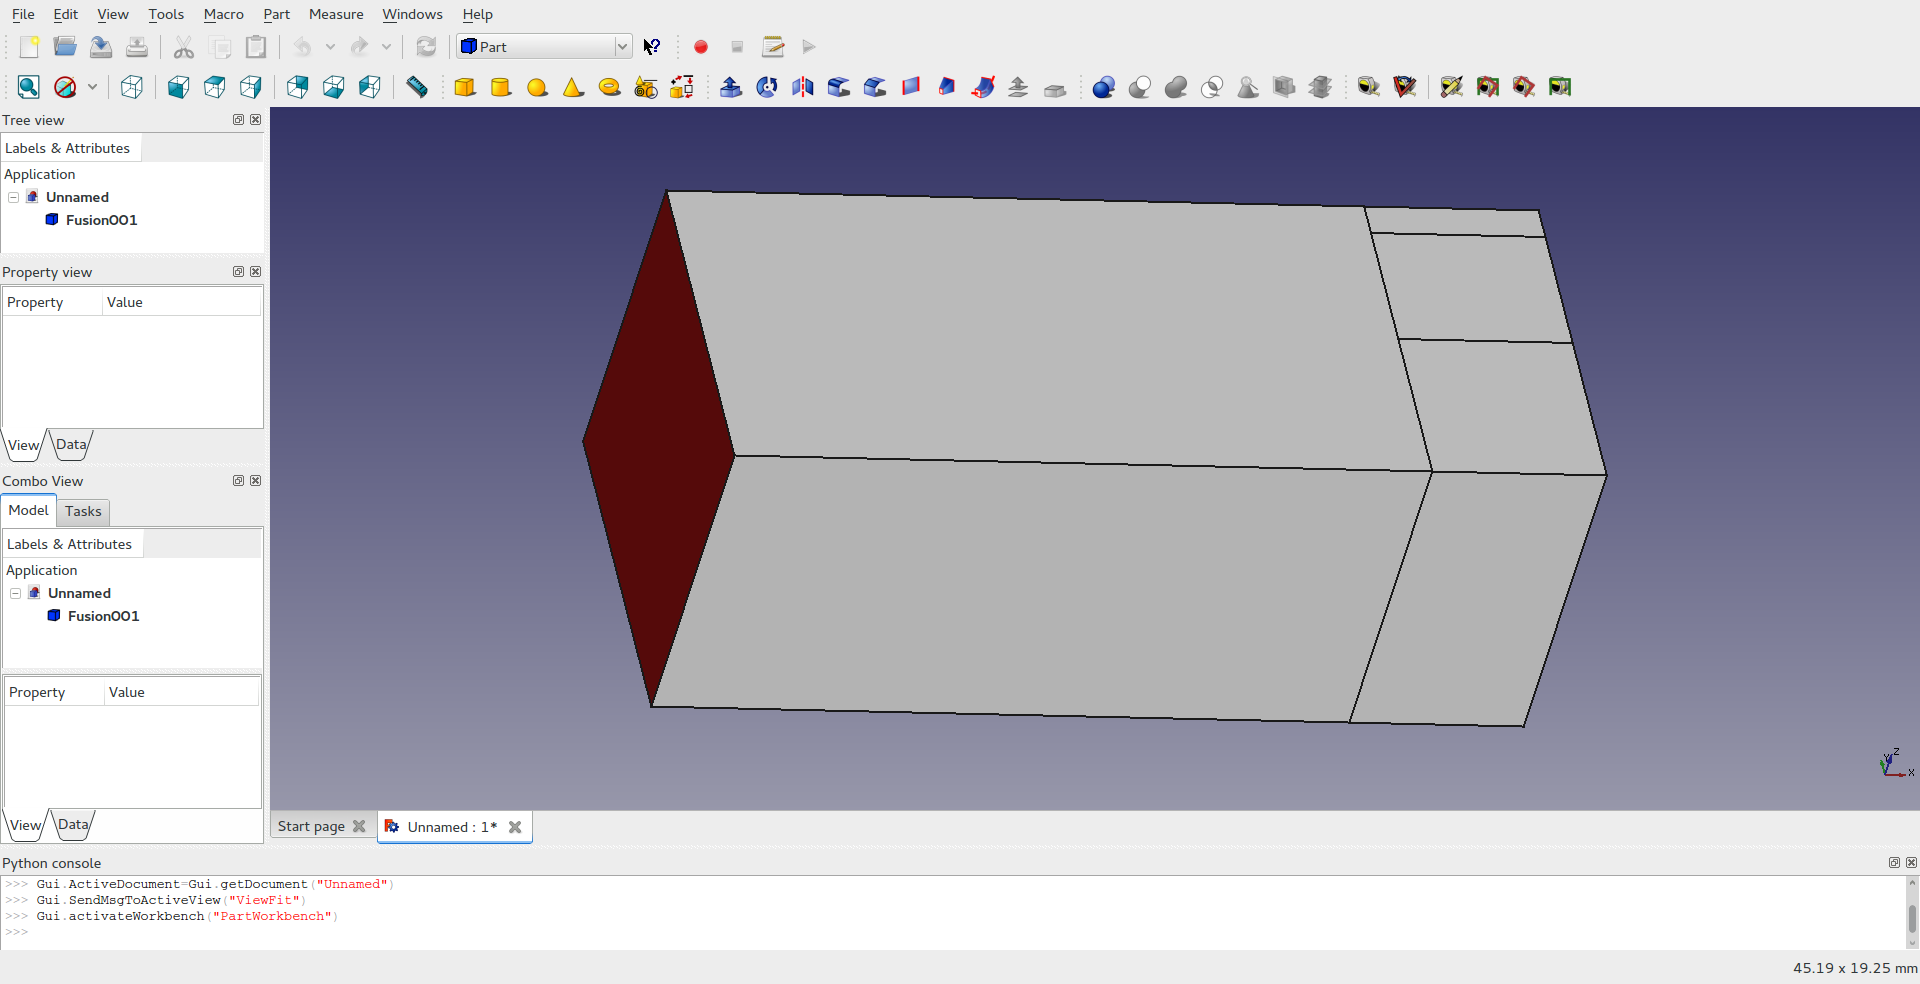
\includegraphics[width=.3\textwidth]{Pictures/TopOp/CantileverFCAD1.png}\hfill
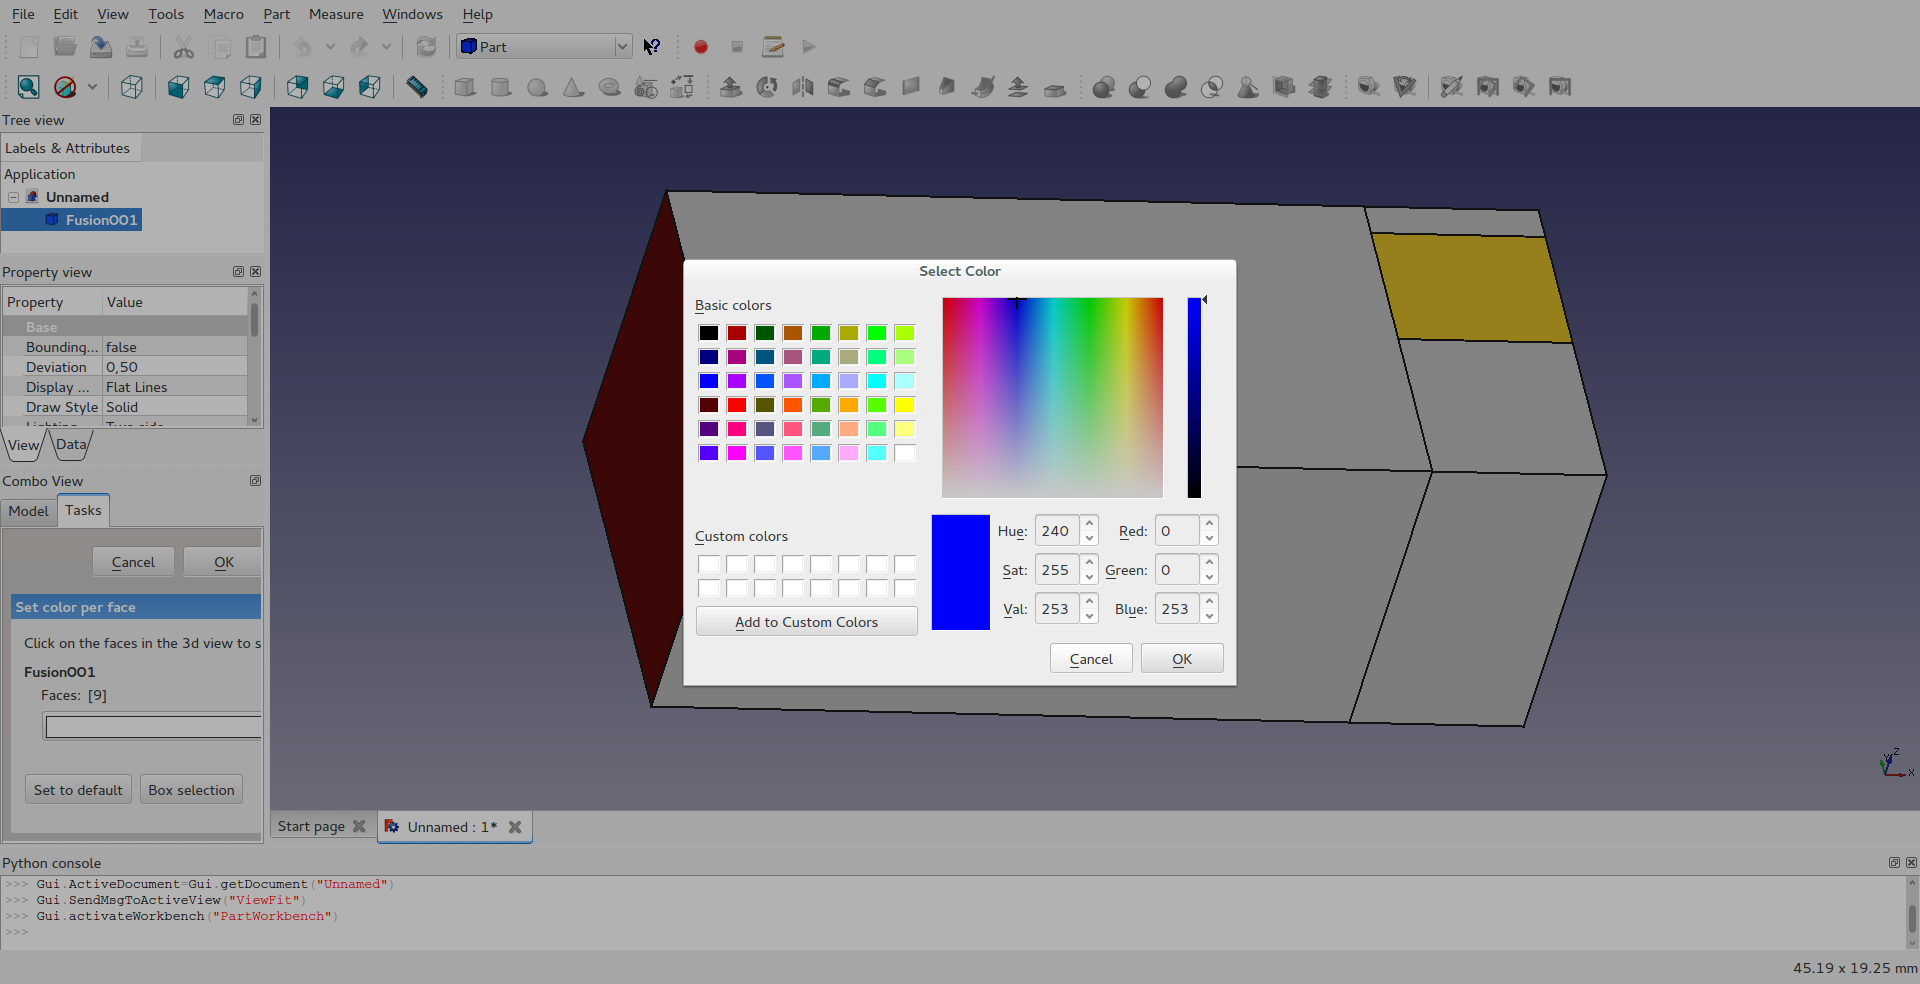
\includegraphics[width=.3\textwidth]{Pictures/TopOp/CantileverFCAD2.png}\hfill
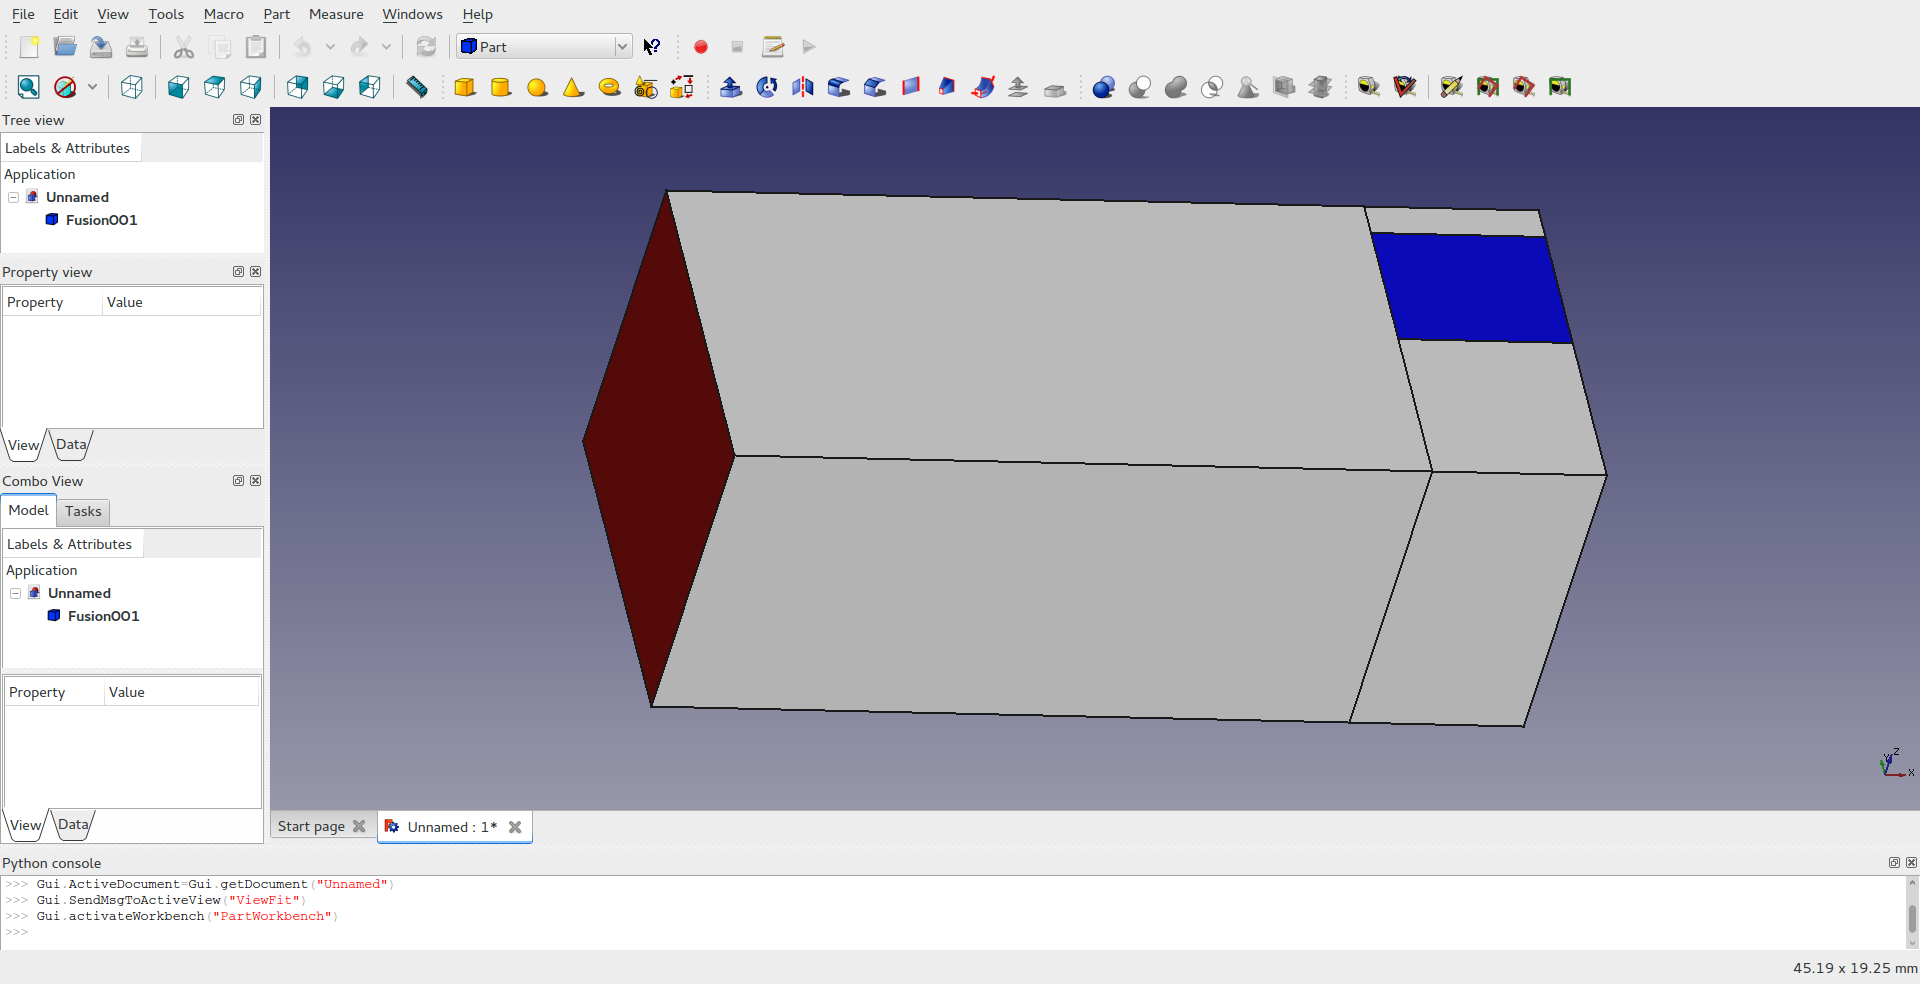
\includegraphics[width=.3\textwidth]{Pictures/TopOp/CantileverFCAD3.png}

\caption{Color faces in FreeCAD}
\label{fig: FreeCADColoring}
\end{figure}
\end{frame}

\subsection{The internal view}
\begin{frame}{The internal view DRAFT}
\begin{itemize}
	\item The pipeline:
	\begin{enumerate}
		\only<1> {
		\item Read STEP and IGES file, extract colours and faces
		\item Voxelize faces using OpenCascade
		\item Calculate index for each voxel for ToPy
		\item Write ToPy input file
		\item Execute ToPy on the input file
		\item Execute Surface Reconstruction on ToPy vtk output
		}		
		\only<2> {
		\item Read STEP and IGES file, extract colours and faces
		\begin{itemize}
			\item STEP file holding the colours
			\item IGES holding the structure
		\end{itemize}
		}
		\only<3> {
		\item Read STEP and IGES file, extract colours and faces
		\item Voxelize faces using OpenCascade
		\begin{itemize}
			\item Included open cascade voxelizer
			\begin{figure}[htp]
				\centering
				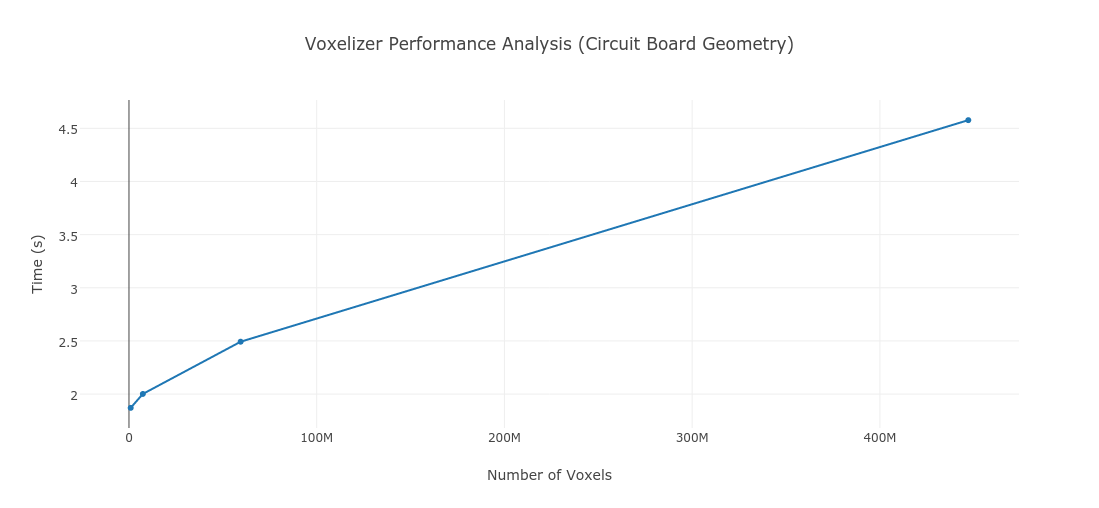
\includegraphics[width=.4\textwidth]{Pictures/TopOp/VoxelizerScalingPlot.png}
				\caption{Scaling of voxelizer}
				\label{fig: VoxelScaler}
			\end{figure}
		\end{itemize}
		}
		\only<4> {
		\item Read STEP and IGES file, extract colours and faces
		\item Voxelize faces using OpenCascade
		\item Calculate index for each voxel for ToPy
		\begin{itemize}
			\item Different indexing for elements and nodes in ToPy
			\begin{figure}[htp]
				\centering
				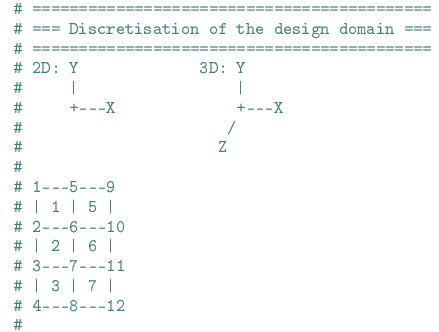
\includegraphics[width=.4\textwidth]{Pictures/TopOp/ToPyIndexing.png}
				\caption{Indexing in ToPy}
				\label{fig: TopyIndex}
			\end{figure}
		\end{itemize}
		}
		\only<5> {
		\item Read STEP and IGES file, extract colours and faces
		\item Voxelize faces using OpenCascade
		\item Calculate index for each voxel for ToPy
		\item Write ToPy input file
		\begin{itemize}
			\item Each voxelindex is specifically written
			\begin{figure}[htp]
				\centering
				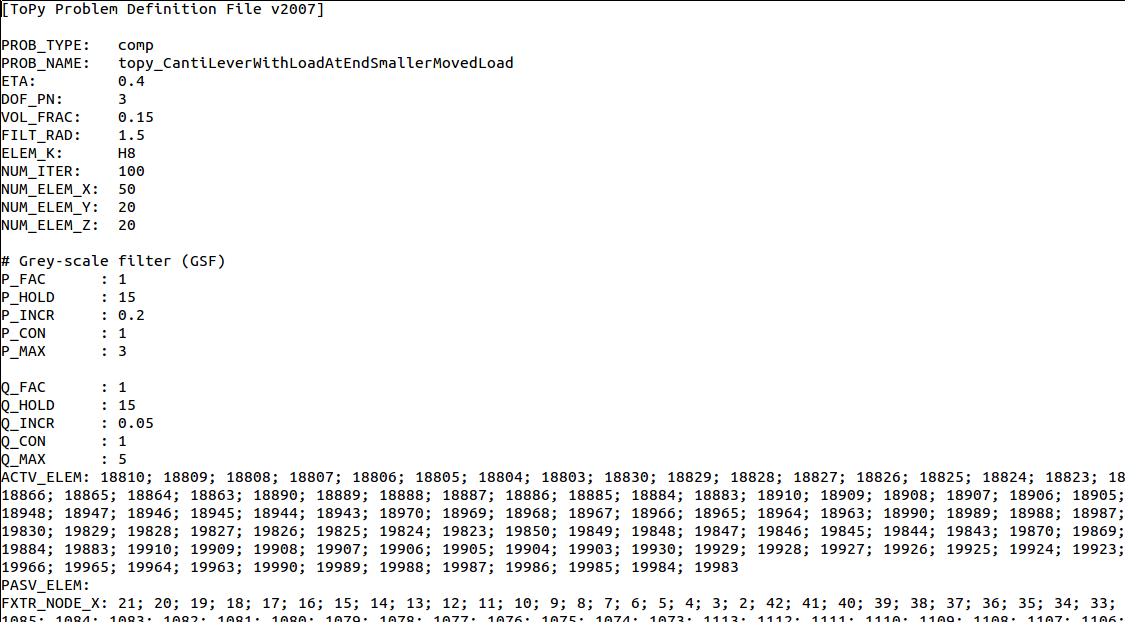
\includegraphics[width=.4\textwidth]{Pictures/TopOp/ToPyInput.png}
				\caption{Script for ToPy}
				\label{fig: TopyScript}
			\end{figure}
		\end{itemize}
		}
		\only<6> {
		\item Read STEP and IGES file, extract colours and faces
		\item Voxelize faces using OpenCascade
		\item Calculate index for each voxel for ToPy
		\item Write ToPy input file
		\item Execute ToPy on the input file
		\begin{itemize}
			\item Topy runs....
			\begin{figure}[htp]
				\centering
				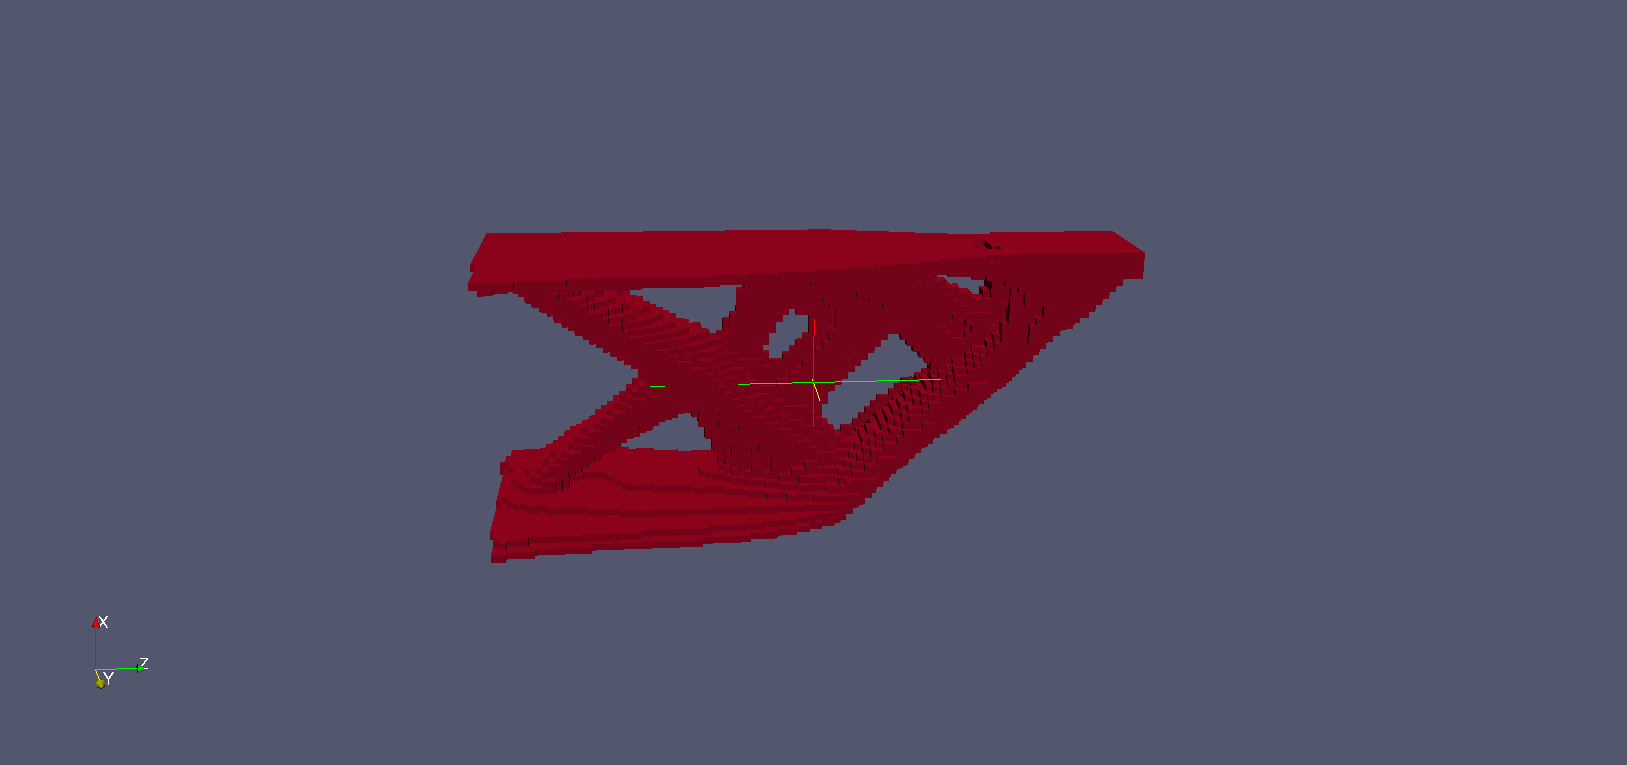
\includegraphics[width=.4\textwidth]{Pictures/TopOp/CantileverToPy.png}
				\caption{ToPy Output}
				\label{fig: topyoutput}
			\end{figure}
		\end{itemize}				
		}
		\only<7> {
		\item Read STEP and IGES file, extract colours and faces
		\item Voxelize faces using OpenCascade
		\item Calculate index for each voxel for ToPy
		\item Write ToPy input file
		\item Execute ToPy on the input file
		\item Execute Surface Reconstruction on ToPy vtk output
		\begin{itemize}
			\item Running dual contouring algorithm
			\item add Picture
		\end{itemize}				
		}
	\end{enumerate}
\end{itemize}

\end{frame}